\documentclass[titlepage]{tufte-book}

\usepackage[runall=true]{pythontex}
\setpythontexworkingdir{<outputdir>}
\usepackage{environ}
\usepackage{morewrites}
\usepackage{amsthm}
\usepackage{amsmath}
\usepackage{amssymb}
\usepackage[pdftex]{graphicx}
\usepackage{epstopdf}
\usepackage{hyperref}
\usepackage{alltt}
\usepackage{listings}
\usepackage{array}
\usepackage{extarrows}
\usepackage{setspace}
\usepackage{tikz}
\usepackage{tikz-qtree}
\usetikzlibrary{calc}
\usetikzlibrary{positioning}
\usepackage{hyperref}
\usepackage{graphviz}
\usepackage{geometry}                % See geometry.pdf to learn the layout options. There are lots.
\usepackage{bashful}
\usepackage{microtype} % Improves character and word spacing
\usepackage{caption}

\usepackage{booktabs} % Better horizontal rules in tables

\setkeys{Gin}{width=\linewidth,totalheight=\textheight,keepaspectratio} % Improves figure scaling
\graphicspath{{figures/}}

\usepackage{fancyvrb} % Allows customization of verbatim environments
\fvset{fontsize=\normalsize} % The font size of all verbatim text can be changed here

\newcounter{problem}
\newcounter{total}
\newcommand{\step}[1]{{}
\vspace{4pt} \noindent {\bf \theproblem. }#1\addtocounter{problem}{1}}

\newcommand{\cut}[1]{}

\usepackage[tikz]{bclogo}
\usepackage{tikz}
\usetikzlibrary{calc}

\lstdefinestyle{BashInputStyle}{
  language=bash,
  basicstyle=\small\ttfamily,
  numberstyle=\tiny,
  showstringspaces=false,
  numbersep=3pt,
  otherkeywords={|, ;, ', ", *,>, <, *, &, `, $},
  alsoletter={:~_},
  columns=fullflexible,
  backgroundcolor=\color{yellow!20},
  linewidth=0.93\linewidth,
  xleftmargin=0.03\linewidth,
  keywordstyle=\color{blue},
  emph={ls, cat, head, tail, more, less, sort, uniq, kill java, grep, zip, unzip, tar, wc, cp, chmod,chown},
  emphstyle=\color{black}\bfseries,
    commentstyle=\color{gray}\slshape
    }

\newcommand{\chili}{\scalebox{.04}{
\includegraphics{figures/chili.pdf}}}
\newcommand{\chchili}{{\chili\chili}}
\newcommand{\chchchili}{{\chchili\chili}}

% The units package provides nice, non-stacked fractions and better spacing
% for units.
\usepackage{units}

% The fancyvrb package lets us customize the formatting of verbatim
% environments.  We use a slightly smaller font.
\usepackage{fancyvrb}
\fvset{fontsize=\normalsize}

% Small sections of multiple columns
\usepackage{multicol}

\hypersetup{
urlcolor=blue,
colorlinks=true
}
\usepackage[noline, procnumbered, linesnumberedhidden, boxed]{algorithm2e}

\newcommand{\openepigraph}[2]{ % This block sets up a command for printing an epigraph with 2 arguments - the quote and the author
\begin{fullwidth}
\sffamily\large
\begin{doublespace}
\noindent\allcaps{#1}\\ % The quote
\noindent\allcaps{#2} % The author
\end{doublespace}
\end{fullwidth}
}

\newcommand{\figref}[1]{Figure~\ref{#1}}
\renewcommand{\thefigure}{\arabic{figure}}

\newenvironment{callout}[1]{
\[
  \left[
      \begin{tabular}{@{\quad}m{.05\textwidth}@{\qquad}m{.75\textwidth}@{\quad}}
        \scalebox{1.5}{#1} & 
          \raggedright%
}
{
      \end{tabular}
    \right]
\]
}

\newcommand{\blankpage}{\newpage\hbox{}\thispagestyle{empty}\newpage} % Command to insert a blank page

\usepackage{makeidx} % Used to generate the index
\makeindex % Generate the index which is printed at the end of the document

\renewcommand{\maketitlepage}[0]{%
  \cleardoublepage%
  {%
  \sffamily%
  \begin{fullwidth}%
  ~
  \vspace{11.5pc}%
  \fontsize{36}{40}\selectfont\par\noindent\textcolor{darkgray}{\allcaps{\thanklesstitle}}%
  
\scalebox{.2}{
\includegraphics{figures/msan-logo}}
  \vspace{11.5pc}%
  \fontsize{12}{18}\selectfont\par\indent\textcolor{darkgray}{\allcaps{\thanklessauthor}\\
\indent{\tt parrt@cs.usfca.edu}\\
\href{http://parrt.cs.usfca.edu}{http://parrt.cs.usfca.edu}}%
  \vspace{11.5pc}%
  \fontsize{14}{16}\selectfont\par\noindent\allcaps{\thanklesspublisher}%
  \end{fullwidth}%
  }
  \thispagestyle{empty}%
  \clearpage%
}

\titlecontents{part}% FIXME
    [0em] % distance from left margin
    {\vspace{1.5\baselineskip}\begin{fullwidth}\LARGE\rmfamily\itshape} % above (global formatting of entry)
    {\contentslabel{2em}} % before w/label (label = ``II'')
    {} % before w/o label
    {\rmfamily\upshape\qquad\thecontentspage} % filler + page (leaders and page num)
    [\end{fullwidth}] % after

  \titlecontents{chapter}%
    [0em] % distance from left margin
    {\vspace{1.5\baselineskip}\begin{fullwidth}\Large\rmfamily\itshape} % above (global formatting of entry)
    {\hspace*{0em}\contentslabel{2em}} % before w/label (label = ``2'')
    {\hspace*{4em}} % before w/o label
    {\rmfamily\upshape\qquad\thecontentspage} % filler + page (leaders and page num)
    [\end{fullwidth}] % after

\titlespacing*{\chapter}{0pt}{0pt}{30pt}
\titlespacing*{\section}{0pt}{3.5ex plus 1ex minus .2ex}{2.3ex plus .2ex}
\titlespacing*{\subsection}{0pt}{3.25ex plus 1ex minus .2ex}{1.5ex plus.2ex}

\begin{document}

\chapter{Approximating $\sqrt{n}$ with the Babylonian Method}

\setcounter{problem}{1}
\section{Motivation}

\begin{fullwidth}

This lab shows how to encode and solve a recurrence relation from mathematics using iteration in Python to approximate a real-world, real valued function.  It also teaches how to quickly prototype something in Excel (if warranted).
 
\section{Discussion}

To approximate square root, $\sqrt{n}$, the idea is to pick an initial estimate, $x_0$, and then iterate with better and better estimates, $x_{i}$, using the recurrence relation:

\[
x_{i+1} = \frac{1}{2} (x_i + \frac{n}{x_i})
\]

To see how this works, jump into Excel (yes, a spreadsheet) and crank through a few iterations by defining cells with $n$ and your initial estimate $x_0$, which can be anything you want. (It's sometimes easier to play around without having to deal with a programming language.) Then you need to define a cell that computes the above better approximation using $x_i$ as the cell above it. I hardcoded the names in column A and the first two rows of column B. Cell B3 should be a formula that computes B4 based upon B3. Then you can extend the formula down and watch it converge on the final (correct) value for $\sqrt{125348}$. My spreadsheet looks like this:

~\\
\scalebox{.25}{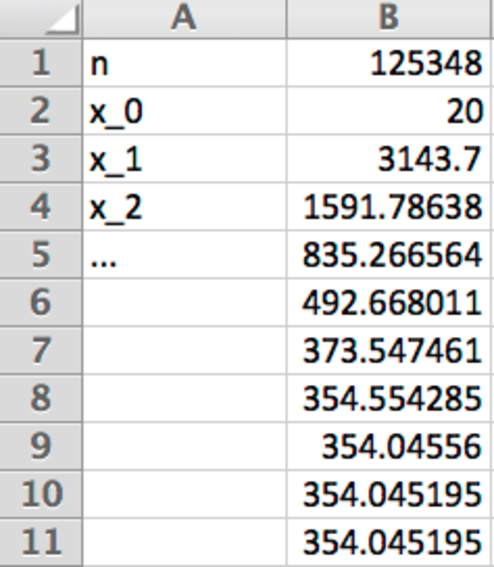
\includegraphics{figures/sqrt-excel.pdf}}
~\\

Try out any nonnegative number and you'll see that it still converges, though at different rates.

There's a great deal on the web you can read to learn more about why this process works but it relies on the average (midpoint) of $x$ and $n/x$ getting us closer to $\sqrt{n}$.  It can be shown that if $x$ is above $\sqrt{n}$ then $n/x$ is below $\sqrt{n}$ and the reverse is true if $x$ is below the root.  The iteration converges and does so quickly. Informally, as shown in Wikipedia, we can represent the true square root by adding an error term to our estimate:

\[
\sqrt{n} = x + \epsilon
\]

or,

\[
n = (x + \epsilon)^2
\]

Expanding, we get:

\[
n = x^2 + 2x\epsilon + \epsilon^2
\]

Solving for $\epsilon$:

\[
n - x^2 = \epsilon (2x + \epsilon)
\]

\[
\epsilon = \frac{n - x^2}{2x + \epsilon}
\]

Because $\epsilon$ is much smaller than $x$, we can drop it from the denominator leaving us with an estimate of epsilon:

\[
\epsilon = \frac{n - x^2}{2x}
\]

Then we can plug it back into $x + \epsilon$ and get:

\[
x := x + \epsilon = x + \frac{n - x^2}{2x} = \frac{2x^2}{2x} + \frac{n - x^2}{2x} = \frac{1}{2}\frac{x^2 + n}{x} = \frac{1}{2}(x + \frac{n}{x})
\]

Which gets its back to the Babylonian formula. Since we dropped an $\epsilon$ term, this formula for $x$ is inexact but it gets us closer to $\sqrt{n}$.

\cut{
To play first use Excel: 
=0.5*(B2+\$B\$1/B2)
}

Now that you understand how this estimate works, your goal is to implement a simple Python method called sqrt() that uses the Babylonian method to approximate the square root. File {\tt sqrt.py} is in you are repository with some starter code. You will also find unit tests in {\tt stats/test\_sqrt.py}, which you can run with:

\begin{lstlisting}[style=BashInputStyle]
$ python -m pytest test_sqrt.py
\end{lstlisting}

\begin{callout}{\bctakecare}
You may not use math.sqrt() for implementing your function, but you may use it for testing the results.  Obviously.
\end{callout}

\begin{callout}{\bcplume}
{\bf Deliverables}. Make sure that {\tt stats/sqrt.py} is correctly committed to your repository and pushed to github. 
\end{callout}

\end{fullwidth}


\end{document}
